\begin{figure}[t]
\centering
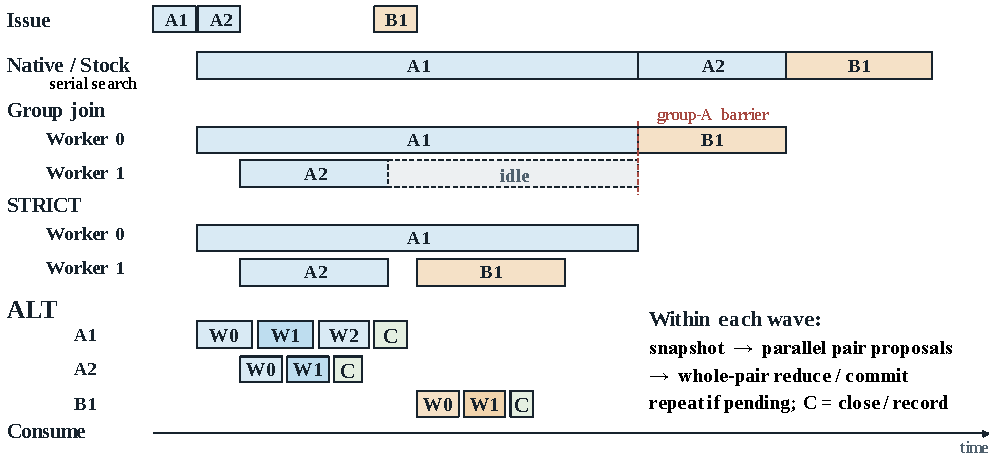
\includegraphics[width=\columnwidth]{figures/timeline.pdf}
\caption{Illustrative schedules for samples $A_1,A_2,B_1$. Group waits at the group boundary. STRICT can issue $B_1$ while $A_1$ is active and still consume in native order. Within an ALT sample, $W_i$ denotes a wave and C marks bucket closure.}\label{fig:contracts}
\end{figure}
\begin{figure*}[t]
\centering
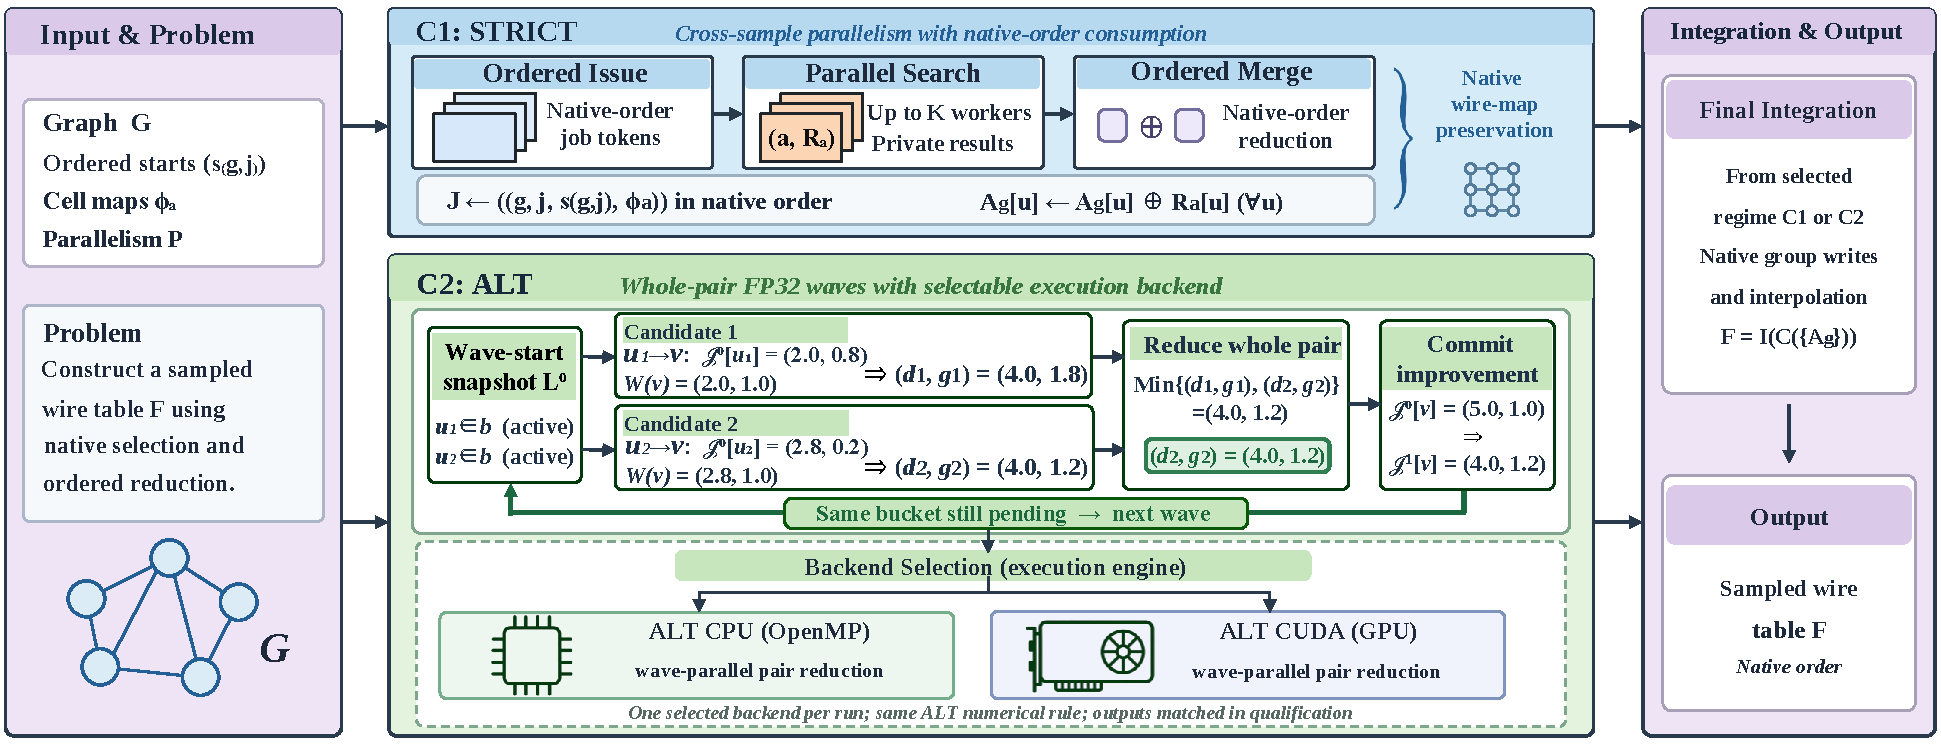
\includegraphics[width=\textwidth]{figures/framework.pdf}
\caption{Layer-aware lookahead construction. In C1, $P$ counts workers and $K$ bounds live tokens. Proposition~\ref{prop:strict} gives the native-map guarantee. C2 distributes samples across CPU workers or processes active nodes in parallel on the GPU (CUDA), using the same whole-pair rule. The selected regime returns sample results for native group writes and interpolation.}\label{fig:framework}
\end{figure*}
